\documentclass{article}

\usepackage{graphicx}
\usepackage{latexsym}

\setlength{\pdfpagewidth}{8.5truein}
\setlength{\pdfpageheight}{11truein}

\def\s{\hbox{s}}
\def\m{\hbox{m}}

\usepackage{fullpage}

\addtolength{\topmargin}{-.5in}
\textheight 9in

\begin{document}

\title{Physics and Math of Music --- Day 4 --- Strings}
\date{Friday, February 15, 2002}
\author{Peter Folk ({\tt pfolk@uni}) and Paul Grayson ({\tt pgrayson@uni})}
\maketitle

\section*{Air is a spring}

Air can be squeezed and stretched, just like the slinky.  This
squeezing and stretching connects all the air together and allows
sound to travel from its source to our ears.

\section*{Spaces full of air are oscillators}

If we have a long closed tube, full of air, it contains a bunch of
oscillators, just like the slinky.  This time, however, instead of
moving up and down, the air is becoming stretched and squeezed.  So
our graph of the possible oscillations shows the left-right motion of
the air, not its up-down motion.

\begin{figure}[h]
\begin{center}
	\input figures/air_harmonics.tex
	\caption{Different harmonics of a closed tube of air.}
\end{center}
\end{figure}

The air doesn't move very much near the ends of the tube, because it
is closed.  But some musical instruments (trumpet, tuba, etc.) are
open at one end, so the air is free to move there!  Then we get
harmonics like this:

\begin{figure}[h]
\begin{center}
	\input figures/air_harmonics_open.tex
	\caption{Different harmonics of an open tube of air.}
\end{center}
\end{figure}

Notice that the second wave has three times the frequency of the
first.  Instead of following the 1,2,3,{...} pattern of the closed
tube, the frequencies of an open tube follow a 1,3,5,{...} pattern.

\section*{We can calculate the frequencies of a tube full of air}
The equations for the frequencies of a tube full of air look almost
identical to those for a pendulum and a slinky:

\begin{tabular}{rl}
Pendulum: & $\displaystyle {1 \over 2\pi} \sqrt{F_{\hbox{\tiny{gravity}}} \over m L}$ \\
Spring: &
 $\displaystyle 1\cdot{1 \over 2} \sqrt{F_{\hbox{\tiny{tension}}} \over m L}\,\,\,\hbox{, }\,\,\,
 2\cdot{1 \over 2} \sqrt{F_{\hbox{\tiny{tension}}} \over m L}\,\,\,\hbox{, }\,\,\,
 3\cdot{1 \over 2} \sqrt{F_{\hbox{\tiny{tension}}} \over m L}\,\,\,\hbox{, ...}$ \\
Closed tube: &
 $\displaystyle 1\cdot{1 \over 2} \sqrt{F_{\hbox{\tiny{pressure}}} \over m L}\,\,\,\hbox{, }\,\,\,
 2\cdot{1 \over 2} \sqrt{F_{\hbox{\tiny{pressure}}} \over m L}\,\,\,\hbox{, }\,\,\,
 3\cdot{1 \over 2} \sqrt{F_{\hbox{\tiny{pressure}}} \over m L}\,\,\,\hbox{, ...}$ \\
Open tube: &
 $\displaystyle 1\cdot{1 \over 4} \sqrt{F_{\hbox{\tiny{pressure}}} \over m L}\,\,\,\hbox{, }\,\,\,
 3\cdot{1 \over 4} \sqrt{F_{\hbox{\tiny{pressure}}} \over m L}\,\,\,\hbox{, }\,\,\,
 5\cdot{1 \over 4} \sqrt{F_{\hbox{\tiny{pressure}}} \over m L}\,\,\,\hbox{, ...}$
\end{tabular}

In the pendulum formula, I used $F_{\hbox{\tiny{gravity}}}/m$ instead
of~$9.8$ so it would look closer to the others.  In the tube formulas,
$F_{\hbox{\tiny{pressure}}}$ is the force of air pressure along the
tube, and {\it m\/} is the mass of the air inside the
tube.  This is just the air pressure~$P$, multiplied by the
cross-sectional area of the tube.

When you press the valves of a trumpet, or open the holes in a
clarinet, you change $L$ and~$m$, which changes the frequency of the
note!

\section*{A real instrument is more complicated!}
The bell of a trumpet affects different frequencies in different ways:

\begin{figure}[h]
\begin{center}
	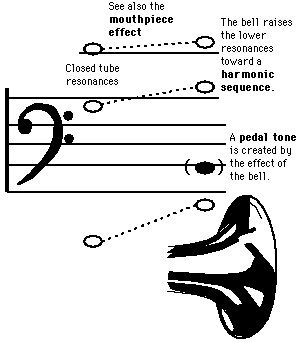
\includegraphics[width=1.5in]{figures/brass.png}
	\caption{How the bell of a trumpet affects its pitch.}
\end{center}
\end{figure}


\footnote{The tube formulas are not exact; you need to correct
(by about 20\%) for the fact that the temperature of the air changes a
little as sound travels through it.}

\end{document}
